\documentclass{article}

\usepackage[T2A]{fontenc}
\usepackage[utf8]{inputenc}
% \usepackage[russian]{babel}
\usepackage{amsmath}
\usepackage{amssymb}
\usepackage{amsthm}
\usepackage{mathrsfs}

\usepackage{dan2e}

\usepackage{hyperref}       % hyperlinks
\usepackage{url}            % simple URL typesetting
\usepackage{booktabs}       % professional-quality tables
\usepackage{amsfonts}       % blackboard math symbols
\usepackage{nicefrac}       % compact symbols for 1/2, etc.
\usepackage{microtype}      % microtypography
\usepackage{lipsum}		% Can be removed after putting your text content
\usepackage{graphicx}
% \usepackage{natbib}
% \usepackage{doi}
\usepackage{mathtools}
\usepackage{xspace}	
\usepackage{amsthm}
\usepackage{setspace}
\usepackage{comment}
\usepackage{amsmath,amssymb}
\usepackage{algorithm}
\usepackage{algpseudocode}
\theoremstyle{definition}
\newtheorem{defi}{Определение}
\theoremstyle{plain}
% \newtheorem{remark}{Замечание}
% \newtheorem{theorem}{Теорема}

\newtheorem{lemma}{Лемма}

% my addition


\usepackage[english, russian]{babel}
\usepackage[backend=biber,style=ieee,autocite=inline]{biblatex}
\bibliography{refs.bib}
\DefineBibliographyStrings{english}{%
  bibliography = {References},}
\DeclareFieldFormat{doi}{%
  doi\addcolon\space
  \ifhyperref
    {\lowercase{\href{https://doi.org/#1}{\nolinkurl{#1}}}}
    {\lowercase{\nolinkurl{#1}}}
}

\usepackage{graphicx}
\usepackage[symbol]{footmisc}
\renewcommand{\thefootnote}{\fnsymbol{footnote}}
\usepackage{float}
\usepackage{mathtools}
\usepackage{amssymb, amsmath, latexsym}
\usepackage{nicefrac}
\usepackage{hhline}
\usepackage{makecell}
\usepackage{caption}
\usepackage{multirow}
\renewcommand\theadalign{bc}
\renewcommand\theadfont{\bfseries}
\renewcommand\theadgape{\Gape[2pt]}
\renewcommand\cellgape{\Gape[2pt]}

\usepackage{colortbl}
\definecolor{bgcolor}{rgb}{0.8,1,1}
\definecolor{bgcolor2}{rgb}{0.8,1,0.8}
\usepackage{threeparttable}
\newcommand{\myred}[1]{{\color{red}#1}}
\newcommand{\myblue}[1]{{\color{blue}#1}}
% \usepackage[nocompress]{cite}
\usepackage{pifont}% http://ctan.org/pkg/pifont
\newcommand{\cmark}{\ding{51}}%
\newcommand{\xmark}{\ding{55}}%
\usepackage[colorinlistoftodos,bordercolor=orange,backgroundcolor=orange!20,linecolor=orange,textsize=scriptsize]{todonotes}
\usepackage{algorithm}\usepackage{algpseudocode}
\newcommand{\argmin}{\mathop{\arg\!\min}}
\newcommand{\argmax}{\mathop{\arg\!\max}}
\allowdisplaybreaks
\graphicspath{ {images/} }
% Used for displaying a sample figure. If possible, figure files should
% be included in EPS format.
%
% If you use the hyperref package, please uncomment the following line
% to display URLs in blue roman font according to Springer's eBook style:
% \renewcommand\UrlFont{\color{blue}\rmfamily}


% my addition end


\begin{document}

% TITLE START
% Перевод данных об алгоритмах
  \renewcommand{\listalgorithmname}{Список алгоритмов}
  \floatname{algorithm}{Алгоритм}
\Volume{--}
\Year{2023}
\Pages{--}

\udk{--}

\title{Оптимальное разделение данных в распределенной оптимизации для машинного обучения}

\author{Медяков Даниил\Addressmark[1],
Молодцов Глеб\Addressmark[1],
Александр Безносиков\Addressmark[1],
Александр Гасников\Addressmark[1]}

\Addresstext[1]{Московский физико-технический институт, Долгопрудный, Россия}

\Emailtext[1]{mediakov.do@phystech.edu}

\markboth{Д. Медяков, Г. Молодцов, А. Безносиков, А. Гасников}{Оптимальное разделение данных в распределенной оптимизации для машинного обучения}


% \presentedby{Представлено академиком Б.\,С.~Кашиным}

% \dateA{01.04.2022}
% \dateB{31.04.2022}
% \dateC{27.05.2022}


% \alttitle{Generalization of Landau and Becker--Pommerenke inequalities}

% \altauthor{O.\,S.~Kudryavtseva\Addressmark[a,b]\Emailmark[1], A.\,P.~Solodov\Addressmark[a]\Emailmark[2]}

% \altAddresstext[a]{Lomonosov Moscow State University, Moscow Center for Fundamental and Applied Mathematics, \\ Moscow, Russian Federation}

% \altAddresstext[b]{Volgograd State Technical University, Volgograd, Russian Federation}

% \altpresentedby{Presented by Academician of the RAS B.\,S.~Kashin}



\maketitle

% \doi{10.31857/S2686954322040117}

% ABSTRACT STARTS

\begin{abstract}
Задача распределенной оптимизации в последнее время становится все более актуальной. Эта постановка имеет множество преимуществ, например, обработка большого объема данных за меньшее время по сравнению с нераспределенными методами. Однако, большинство распределенных подходов страдают от существенного недостатка -- большой стоимости коммуникаций. Поэтому в последнее время большое количество исследований было направлено на решение этой проблемы. Один из таких подходов использует локальное сходство данных. В частности, существует алгоритм, доказательно оптимально использующий свойство подобия.. Однако этот результат, а также результаты других работ устраняют проблему коммуникаций, фокусируясь только на том факте, что они значительно дороже локальных вычислений и не учитывает различные мощности устройств в сети и различное соотношение между временем коммуникаций и затртами на локальные вычисления. Такая проблема и рассматривается в данном исследовании, целью которого является достижение оптимального распределения данных между сервером и локальными машинами при любой стоимости коммуникаций и локальных вычислений. Время работы сети сравнивается при равномерном и оптимальном распределених данных. Ускорение, которое получается за счет последнего, подтверждено экспериментально.
\end{abstract}


\section{Вступление}

\section*{1.1. Распределенная оптимизация}

Рассматривается задача оптимизации следующего вида:
\begin{equation}
    \label{eq:1}
    \underset{x\in \mathbb{R}^d}{\min} ~ f(x) = \frac{1}{n} \sum \limits_{i = 1}^{n} f _i(x),
\end{equation}
где $x\in\mathbb{R}^d$ содержит параметры статистической модели для обучения, $n$ -- количество устройств/узлов в сети, а $f_i$ -- эмпирическая функция потерь на $i$-ом устройстве, то есть $f_i(x) = \frac{1}{b_i}\sum_{j = 1}^{b_i} l(x, z_i^j)$, с $z_i^1, \ldots ,z_i^{b_i}$ - набором выборок $b_i$, принадлежащих $i$-му устройству, и $l(x, z_i^j)$ измеряет несоответствие между параметром $x$ и образцом $z_i^j$. Это формулировка задачи распределенной оптимизации. В настоящее время есть несколько причин сделать такую постановку задачи.

Чтобы достичь наилучших результатов в современных оптимизационных задачах в машинном обучении, исследователи и практики сталкиваются с различными вызовами. Иметь дело с современными моделями машинного обучения остается чрезвычайно сложной задачей, в первую очередь потому, что модели обучаются на все более объемных выборках данных. Наличие обучающей выборки большого объёма в наборе данных повышает устойчивость и обобщаемость полученной модели. В этом случае данные обычно обрабатываются с использованием сети устройств, т.е. собираются распределенным образом и хранятся в крайних узлах сети, например, как при классическом кластеризационном \cite{verbraeken2020survey} и федеративном \cite{konevcny2016federated, li2020federated, kairouz2021advances} обучении.

Для решения задачи \eqref{eq:1} было предложено несколько методов решения. Стандартный подход предполагает чередование локальных вычислений на краевых устройствах (узлах $i = 2, \ldots, n$) с коммуникациями с сервером ($i = 1$), который поддерживает и обновляет актуальную копию оптимизационных переменных, в конечном итоге формируя окончательную оценку решения. При распределенном обучении сложных моделей проблемным местом часто становятся коммуникационные расходы между устройствами в сети. Такая проблема обусловливает необходимость разработки более эффективных методов распределенного обучения, некоторые из которых были описаны в \cite{konevcny2016federated, ghosh2020communication, smith2018cocoa, gorbunov2021marina}.

\section*{1.2. Распределённая оптимизация в условиях схожести данных}

Сегодня в машинном обучении модно использовать методы, основанные на идее инерционного моментума. Одним из путей решения распределенной оптимизационной задачи является применение ускорения Нестерова \cite{nesterov2018lectures}, которое представляет собой оптимальный метод для гладких нераспределенных оптимизационных задач. Для распределенных сетей он может быть применен следующим образом. На каждой итерации  локально вычисляется градиент и результаты отправляются на сервер. Он, в свою очередь, усредняет полученные градиенты и делает шаг метода. Тогда количество коммуникаций будет равно количеству итераций. В этом случае  получаются оптимальные оценки для локальных вычислений - $\sqrt{\kappa}, \kappa = \nicefrac{L}{\mu}$, где $L$ и $\mu$ - константы гладкости и сильной выпуклости целевой функции $f$. В случае, когда $\kappa$ мала, такой подход вполне приемлем. Однако для плохо обусловленных функций с большой $\kappa$ полиномиальная зависимость от $\kappa$ может оказаться неудовлетворительной из-за высокой стоимости коммуникаций. Это часто имеет место для многих задач Минимизации Эмпирического Риска (МЭР), когда оптимальный параметр регуляризации для тестового прогнозирования очень мал.

Для дальнейшего решения пробелемы стоимости коммуникаций можно использовать дополнительную структуру, обычно встречающуюся в задачах МЭР, известную как схожесть данных \cite{arjevani2015communication, shamir2014communication, matsushima2014distributed}. Ее можно определить как разность градиентов функций, т.е. $\|\nabla f_i (x) - \nabla f_j (x)\| < \delta ~~ \forall x$. Но такой подход не является "естественным", так как если задача не ограниченна, то такая $\delta$ не может существовать. Рассмотрим, например, квадратичную постановку: $\nexists~ \delta: \|(A_i - A_j)x\| < \delta~$, если $~ x\rightarrow \infty$. Поэтому, сфокусируемся на другом подходе, а именно, на подобии Гессианнов. В частности, для всех $x$ из рассматриваемой области и всех $i \neq j; ~ i,j \in \{1,\ldots,n\}$, разность между матрицами Гессиана локальных потерь, обозначаемая $\|\nabla ^2 f_i(x) - \nabla ^2 f_j(x)\|$, ограничена $\delta$, где $\delta > 0$ измеряет степень сходства. При таком предположении можно оценить $\delta \sim \mathcal O(\nicefrac{1}{\sqrt{N}})$, где $N$ - размер выборки на одно устройство \cite{arjevani2015communication}. Впервые такой подход был исследован в \cite{shamir2014communication}. После этого в \cite{arjevani2015communication} были доказаны нижние оценки для этой задачи, где затраты на коммуникации пропорциональны $\sqrt{\nicefrac{\delta}{\mu}}$. Затем, долгое время исследователи пытались найти методы, позволяющие достичь этих оценок. В частности, были получены такие алгоритмы, как \cite{tian2022acceleration, sun2022distributed, reddi2016aide, hendrikx2020statistically, beznosikov2021distributed}. В 2022 году удалось получить оптимальный метод, который описан в \cite{kovalev2022optimal}. 

\section*{1.3. Различные затраты на коммуникации и локальные вычисления} \label{eq:1.3}

Во всех вышеперечисленных работах авторы выдвигали предположение о том, что коммуникации обходятся значительно дороже локальных вычислений. Более того, в целом в работах по распределенной оптимизации, не только в области схожести Гессианов, делалось такое предположение. Данный вопрос будет рассмотрен с другой стороны, уходя от фиксированных больших коммуникаций и сделав 2 \textbf{предположения}:
\begin{itemize}
    \item [1.] Устройства в сети имеют разную мощность, то есть выполняют локальные вычисления одного и того же объема данных за разное время.
    \item [2.] Отношение коммуникационных затрат к локальному времени вычислений -- величина переменная, которая может быть либо $\ll 1$, либо $\gg1$, либо даже $\sim 1$.
\end{itemize}
При таких предположениях необходим новый подход к задаче распределенной оптимизации, основанный на уже полученных оптимальных алгоритмах. Это приводит к исследуемому в данной статье вопросу.
\begin{center}
    \textit{ Можно ли найти такое распределение данных между устройствами в сети, чтобы сократить реальное время работы оптимального алгоритма} \cite{kovalev2022optimal}\textit{~при любых коммуникационных затратах и времени локальных вычислений?}
\end{center}

На практике сети могут работать в течение длительного времени, и, как следствие, в них могут возникать шумы. Другими словами, стоимость связи и мощность устройств не являются постоянными величинами в течении работы сети. Таким образом, делается еще одно \textbf{предположение}:
\begin{itemize}
    \item [3.] Стоимости связи и мощности устройств задаются как случайные величины, затем на длительное время запускается работа сети и измеряются их математическое ожидание и дисперсия. Поскольку распределение данных по устройствам зависит от постоянных времени связи и мощности устройств, то в реальности оптимальное распределение будет отличаться из-за шума.
\end{itemize}

Поэтому в связи с этим предположением возникает вопрос об измерении погрешности времени работы программы при оптимальном распределении данных.
\section*{1.4. Вклад}

В целом наш вклад заключается в следующем:
\begin{itemize}
    \item \textbf{Обобщение модели вычислений.} Строится общая модель времени вычислений в сетях при распределенной оптимизации. Модель основана на оптимальном алгоритме \cite{kovalev2022optimal} и учитывает разницу в мощностях устройств при различных затратах на связь.
    \item \textbf{Всеобъемлющий анализ.} Особое внимание уделяеется частным случаям и полученным в них результатам. Рассматривается случай, когда коммуникации слишком дорогие, а также случай дешёвых коммуникаций (не настолько дорогих, чтобы связь занимала больше времени, чем обработка всех данных одним устройством). Более того, результаты получаются не только с учетом разницы во временных затратах, но и при рассмотрении различных оценок $\delta$.
    \item \textbf{Различные техники получения решения.} Получаются результаты в различных случаях, в том числе для различных оценок $\delta$. Также используются следующие методы: формула Кардано, верхние оценки в предельных случаях и нахождение нуля функции простейшими численными методами.
    \item \textbf{Погрешность решения из-за шума.} При третьем предположении приводена теоретическую погрешность времени работы программы при шуме времени коммуникаций и локальных\\ вычислений.
    \item \textbf{Эксперименты.} На основе проведенных экспериментов было получено подтверждение того, что с выведенным распределением решение выбранной задачи занимает меньшее время. Кроме того, соответствующие эксперименты были дополнены шумом в сети.
\end{itemize}

\section{Постановка задачи}

На данном этапе остановимся на первых двух предположениях из Секции 1.3. Для достижения меньшей коммуникационной и локально-градиентной сложности обратимся к алгоритму \ref{alg:1} из \cite{kovalev2022optimal}. Для этого необходимо представить функцию в виде суммы гладкой выпуклой функции $f_1$ и гладкой потенциально невыпуклой функции $f - f_1$. Тогда алгоритм будет переписан в следующем более общем виде:

\begin{algorithm}
\caption{Accelerated Extragradient}\label{alg:1}
\begin{algorithmic}
\item [1:] \textbf{Input:} $x^0 = x_f^0\in\mathbb R^d$
\item [2:] \textbf{Parameters:} $\tau\in (0, 1), \eta, \theta, \alpha > 0, K\in \{1, 2, \ldots\}$
\item [3:] \textbf{for~}$k = 0, 1, 2, \ldots, K-1$\textbf{~do}
\item [4:]    $\quad\quad x_g^k = \tau x^k + (1 - \tau)x_f^k$
\item [5:]    $\quad\quad x_f^{k+1} \approx \arg\underset{x\in\mathbb R^d}{\min} [A_{\theta}^k (x) := \langle \nabla (f - f_1)(x_g^k), x - x_g^k \rangle + \frac{1}{2\theta}\|x - x_g^k\|^2 + f_1(x)]$ 
\item [6:] $\quad\quad x^{k+1} = x^k + \eta\alpha(x_f^{k+1} - x^k) - \eta\nabla f(x_f^{k+1})$
\item [7:] \textbf{end for}
\item [8:] \textbf{Output:} $x^K$
\end{algorithmic}
\end{algorithm}

Нам необходимо проанализировать работу этого алгоритма, а именно, выяснить, сколько операций выполняет этот алгоритм за итерацию. В строке 5, при решении подзадачи $\arg\min$, на устройствах выполняется одно локальное вычисление для вычисления $f_i(x_g^k)$, затем одна коммуникация для передачи этих результатов и дополнительные вычисления на сервере для нахождения решения $x_f^{k+1}$. Затем, в строке 6, выполняется одно локальное вычисление и одна коммуникация. Получается выражение для общего времени работы алгоритма. Введем следующие обозначения: $\tau_i$ -- время одного локального вычисления на $i$-ом устройстве, $K$ -- количество итераций, $\tau_{comm}$ -- время одной коммуникации, $k_{some}$ -- дополнительные вычисления центрального узла, $n$ -- количество узлов в сети. С учетом этого общее время работы алгоритма можно записать в виде:
\begin{equation}
    \notag
    T_{sum} = 2\cdot\max(\tau_1, \tau_2, \ldots, \tau_n)\cdot K + 2\cdot K\cdot\tau_{comm} + \tau_1\cdot k_{some}.
\end{equation}

Наша задача - минимизировать время $T_{sum}$. С учетом утверждения \eqref{eq:1} и вида функций $f_i$ представим время $\tau_i$ в виде $\tau_i = \tau_i^{loc}\cdot b_i$, где $\tau_i^{loc}$ - мощность, т.е. время, затрачиваемое $i$-м устройством на обработку единицы информации, поступающей на его вход, а $b_i$ - размер набора данных, поступающего на $i$-е устройство. $b_i$ должно удовлетворять следующим ограничениям: $\sum\limits_{i = 1}^{n} b_i = N$, где $N$ - размер всего набора данных, $\delta = \frac{L}{\sqrt{b_i}}$ или $\delta = \frac{L}{b_i}$ \cite{hendrikx2020statistically}.\\
В итоге была получена следующая задача минимизации:
\begin{equation}
    \label{eq:4}
    \underset{\sum\limits_{i = 1}^{n} b_i = N; \delta = \frac{L}{{b_1}^{\gamma}}}{\min}[ 2\cdot\max(\tau_1^{loc}\cdot b_1, \tau_2^{loc}\cdot b_2, \ldots, \tau_n^{loc}\cdot b_n)\cdot K + 2\cdot K\cdot\tau_{comm} + \tau_1\cdot k_{some}], ~ \gamma \in \{\frac{1}{2}, 1\}.
\end{equation}

\section{Как решить (\ref{eq:4})}

\section*{3.1. Первичная задача минимизации}
В \cite{kovalev2022optimal} представлены оценки $K$ и $k_{some}$, а именно: $2\cdot K = \mathcal O(\max\{1, \sqrt{\frac{\delta}{\mu}}\}\log(\frac{1}{\varepsilon})), $\\ $ k_{some} = \mathcal O(\max\{1, \sqrt{\frac{L}{\delta}}, \sqrt{\frac{\delta}{\mu}}, \sqrt{\frac{L}{\mu}}\}\log(\frac{1}{\varepsilon}))$. 

В таком случае, \eqref{eq:4} принимает вид:

\begin{eqnarray}
    \begin{split}
    \label{eq:5}
        \underset{\sum\limits_{i = 1}^{n} b_i = N; \delta = \frac{L}{{b_1}^\gamma}}{\min}[(\max(\tau_1^{loc}\cdot b_1, \tau_2^{loc}\cdot b_2, \ldots, \tau_n^{loc}\cdot b_n) + \tau_{comm}) \cdot \mathcal O(\max\{1, \sqrt{\frac{\delta}{\mu}}\log(\frac{1}{\varepsilon})\}) 
        \\ + ~
        \tau_1^{loc}\cdot b_1\cdot\mathcal O(\max\{1,\sqrt{\frac{L}{\delta}}, \sqrt{\frac{\delta}{\mu}}, \sqrt{\frac{L}{\mu}}\}\log(\frac{1}{\varepsilon}))] ,  ~ \gamma \in \{\frac{1}{2}, 1\}. \hspace{2.4cm}
    \end{split}
\end{eqnarray}

\section*{3.2. Вспомогательная задача}
Рассматриваем следующую вспомогательную задачу:
\begin{equation}
    \label{eq:6}
    \underset{\sum\limits_{i = 2}^{n} b_i = N}{\min} [\max(\tau_2^{loc}\cdot b_2, \tau_3^{loc}\cdot b_3, \ldots, \tau_n^{loc}\cdot b_n)].
\end{equation}


\begin{lemma}
    \label{l1}
    Решением задачи \eqref{eq:6} является $\overrightarrow{b} = (b_2, b_3, \ldots, b_n)^{T}$, такой что $\tau_2^{loc}\cdot b_2 = \tau_3^{loc}\cdot b_3 = \ldots = \tau_n^{loc}\cdot b_n$.
    \begin{proof}
        
        Не умаляя общности, примем фиксированные значения $\tau_2^{loc}\leq \tau_3^{loc}\leq \ldots \leq \tau_n^{loc}$.
        Затем произвольно выберем $b_2\geq b_3\geq \ldots \geq b_n$.
        Это действительно так, иначе имела бы место ситуация, когда $\exists ~ i \neq j: ~ i, j\in \{2, \ldots, n\} : \max(\tau_i^{loc}\cdot b_i, \tau_j^{loc}\cdot b_j) > \max(\tau_i^{loc}\cdot b_j, \tau_j^{loc}\cdot b_i)$, и, следовательно, распределение было бы неоптимальным. 
        
        Главная цель -- минимизировать функцию $g(\overrightarrow{b}) = \max(\tau_2^{loc}\cdot b_2, \tau_3^{loc}\cdot b_3, \ldots, \tau_n^{loc}\cdot b_n)$. Предположим, что существует такое распределение, что $\exists i \in \{2, \ldots, n\}: g(\overrightarrow{b}^0) = \tau_i^{loc}\cdot b_i^0$ является минимумом, и $\forall j: j \geq 2, j \neq i \hookrightarrow \tau_i^{loc}\cdot b_i^0 > \tau_j^{loc}\cdot b_j^0$. Из этого следует, что $b_i^0 > \frac{\tau_j^{loc}}{\tau_i^{loc}}b_j^0 > \frac{\tau_{j_1}^{loc}}{\tau_i^{loc}}b_{j_1}^0 > \ldots > \frac{\tau_{j_k}^{loc}}{\tau_i^{loc}}b_{j_k}^0$. 
        
        Далее, учитывая $\sum\limits_{i = 2}^n b_i = N \hookrightarrow b_i^0 + \frac{\tau_j^{loc}}{\tau_i^{loc}}b_j^0 + \frac{\tau_{j_1}^{loc}}{\tau_i^{loc}}b_{j_1}^0 + \ldots + \frac{\tau_{j_k}^{loc}}{\tau_i^{loc}}b_{j_k}^0 > N$,
        получаем $b_i^0 > N(1 + \tau_i^{loc}\sum\limits_{\substack{j = 2 \\ j \neq i}}^n \frac{1}{\tau_j^{loc}})^{-1}$. Затем рассмотрим $b_i = N(1 + \tau_i^{loc}\sum\limits_{\substack{j = 2 \\ j \neq i}}^n \frac{1}{\tau_j^{loc}})^{-1}, \quad b_j = \frac {\tau_i^{loc}}{\tau_j^{loc}}\cdot b_i  ~~ \forall j \in \{2,\ldots,n\}$. Такое распределение дает минимум $g(\overrightarrow{b}) = \tau_i^{loc}\cdot b_i = \tau_j^{loc}\cdot b_j ~~ \forall j \in \{2,\ldots,n\}$, и $g(\overrightarrow{b}) < g(\overrightarrow{b}^0)$. Это противоречит предположению о минимальности. Таким образом, для распределения, минимизирующего функцию $g(\overrightarrow{b}) = \max(\tau_2^{loc}\cdot b_2, \tau_3^{loc}\cdot b_3, \ldots, \tau_n^{loc}\cdot b_n)$, справедливо $\tau_2^{loc}\cdot b_2 = \tau_3^{loc}\cdot b_3 = \ldots = \tau_n^{loc}\cdot b_n$.
    \end{proof}
\end{lemma}
Вернемся к задаче \eqref{eq:5}. Помимо минимального выражения, уже изученного в \eqref{eq:6}, в задаче \eqref{eq:5} имеются дополнительные члены.  $\delta$ в \eqref{eq:5} зависит от величины $b_1$, но не зависит от $b_i, i = \overline{2, n}$. Отсюда и из леммы \ref{l1} следует, что в исходной задаче \eqref{eq:5} обмен данными между 2-м, 3-м и последующими устройствами должен быть пропорциональным. Таким образом, задача \eqref{eq:5} сводится к новой задаче с дополнительными ограничениями:


\begin{eqnarray}
    \begin{split}
    \label{eq:7}
        \min_{\substack{\sum\limits_{i = 1}^{n} b_i = N; \delta = \frac{L}{{b_1}^\gamma};  \\
        \tau_2^{loc}\cdot b_2 = \ldots = \tau_n^{loc}\cdot b_n }} 
        [(\max(\tau_1^{loc}\cdot b_1, \tau_2^{loc}\cdot b_2, \ldots , \tau_n^{loc}\cdot b_n) + \tau_{comm})\cdot \mathcal O(\max\{1, \sqrt{\frac{\delta}{\mu}}\log(\frac{1}{\varepsilon})\})
        \\ + ~
        \tau_1^{loc}\cdot b_1\cdot\mathcal O(\max\{1,\sqrt{\frac{L}{\delta}}, \sqrt{\frac{\delta}{\mu}}, \sqrt{\frac{L}{\mu}}\}\log(\frac{1}{\varepsilon}))] ,  ~ \gamma \in \{\frac{1}{2}, 1\}. \hspace{2.4cm}
    \end{split}
\end{eqnarray}

    

\section*{3.3. Определим окончательную задачу минимизации}
Из леммы \ref{l1} следует, что $b_i\cdot \tau_i^{loc} = const ~ \forall i \in \overline{2, n}$.
Таким образом, $$ N - b_1 = \sum\limits_{i = 2}^{n} b_i = \sum\limits_{i = 2}^{n} \frac{\tau_2^{loc}\cdot b_2}{\tau_i^{loc}} = \tau_2^{loc}\cdot b_2 \cdot \sum\limits_{i = 2}^{n} \frac{1}{\tau_i^{loc}} \Rightarrow
b_2 = \frac{N - b_1}{\tau_2 ^{loc}}(\sum\limits_{i = 2}^{n} \frac{1}{\tau_i^{loc}})^{-1}.$$

Как уже говорилось ранее, рассматривается случай $\delta = \frac{L}{b_1}$ и case of $\delta = \frac{L}{\sqrt{b_1}}$.

\section*{3.3.1. Случай $\delta = \frac{L}{b_1}$}

Здесь выполняются следующие соотношения:
\begin{equation}
    \notag
    \gamma = 1, ~ \mu \leq \delta \leq L \Rightarrow 
    \\
    \notag
    \begin{cases}
      2\cdot K =  \mathcal O(\sqrt{\frac{L}{\mu b_1}}\log(\frac{1}{\varepsilon}))\\
      k_{some} = \mathcal O(\sqrt{\frac{L}{\mu}}\log(\frac{1}{\varepsilon}))
    \end{cases}\,.
\end{equation}

Подставив эти оценки в \eqref{eq:7}, задача примет следующий вид:
\begin{equation}
    \notag
    \underset{\sum\limits_{i = 1}^{n} b_i = N}{\min}[(\max\{\tau_1^{loc}\cdot b_1, \tau_2^{loc}\cdot b_2\} + \tau_{comm}) \cdot \mathcal O(\sqrt{\frac{L}{\mu {b_1}}}\log(\frac{1}{\varepsilon})) + \tau_1^{loc}\cdot b_1 \cdot \mathcal O(\sqrt{\frac{L}{\mu}}\log(\frac{1}{\varepsilon}))].
\end{equation}

В результате, оставив в функции единственную переменную $b_1$, осуществляется переход к окончательному виду задачи минимизации:

\begin{eqnarray}
    \begin{split}
    \label{eq:fm1}
        \underset{0 < b_1 \leq N}{\min}[(\max\{\tau_1^{loc}\cdot b_1; ~(N-b_1) \cdot (\sum\limits_{i = 2}^{n} \frac{1}{\tau_i^{loc}} )^{-1}\} + \tau_{comm}) \cdot \mathcal O(\sqrt{\frac{L}{\mu b_1}}\log(\frac{1}{\varepsilon})) ~+
        \\ + ~
        \tau_1^{loc}\cdot b_1 \cdot \mathcal O(\sqrt{\frac{L}{\mu}}\log(\frac{1}{\varepsilon}))]. \hspace{3.7cm}
    \end{split}
\end{eqnarray}

Исследуем эту задачу далее. Для этого найдем точку, в которой выражения под максимумом совпадают. 
\begin{equation}
    \notag
    b_1^0 \cdot (\tau_1^{loc} + (\sum\limits_{i = 2}^{n} \frac{1}{\tau_i^{loc}})^{-1}) = N (\sum\limits_{i = 2}^{n} \frac{1}{\tau_i^{loc}})^{-1} \Rightarrow b_1^0 = \frac{N (\sum\limits_{i = 2}^{n} \frac{1}{\tau_i^{loc}})^{-1}}{\tau_1^{loc} + (\sum\limits_{i = 2}^{n} \frac{1}{\tau_i^{loc}})^{-1}}.
\end{equation}

Таким образом, получились два полуинтервала, на каждом из которых можно сформулировать свою задачу минимизации:
\begin{eqnarray*}
    \begin{cases}
    (a) ~ ~ 0 < b_1 \leq b_1^0 \Rightarrow \max\{\tau_1^{loc}\cdot b_1; ~(N-b_1) \cdot (\sum\limits_{i = 2}^{n} \frac{1}{\tau_i^{loc}} )^{-1}\} = 
    (N-b_1) \cdot (\sum\limits_{i = 2}^{n} \frac{1}{\tau_i^{loc}})^{-1}
    \\
    (b) ~ ~ b_1^0 <  b_1 \leq N \Rightarrow \max\{\tau_1^{loc}\cdot b_1; ~(N-b_1) \cdot (\sum\limits_{i = 2}^{n} \frac{1}{\tau_i^{loc}} )^{-1}\} = \tau_1^{loc}\cdot b_1
    \end{cases}\,.
\end{eqnarray*}

Строим функции одной переменной $\mathcal{F}_1(b_1), \mathcal{F}_2(b_1)$ на соответствующих полуинтервалах, которые необходимо минимизировать в соответствии с задачей \eqref{eq:fm1}.
\begin{eqnarray*}
    \begin{cases}
(a): ~\mathcal{F}_1(b_1) = [N (\sum\limits_{i = 2}^{n} \frac{1}{\tau_i^{loc}})^{-1} + \tau_{comm}]\cdot 
c_1 \sqrt{\frac{L}{\mu}}\log (\frac{1}{\varepsilon})  b_1^{-\frac{1}{2}} - 
c_1  \sqrt{\frac{L}{\mu}}\log (\frac{1}{\varepsilon})(\sum\limits_{i =
2}^{n} \frac{1}{\tau_i^{loc}})^{-1} b_1^{\frac{1}{2}}  + \tau_1^{loc}\cdot c_2  \sqrt{\frac{L}{\mu}}\log (\frac{1}{\varepsilon}) b_1  \\
(b): ~\mathcal{F}_2(b_1) = \tau_{comm}\cdot 
c_1 \sqrt{\frac{L}{\mu}}\log (\frac{1}{\varepsilon})  b_1^{-\frac{1}{2}} + 
c_1  \sqrt{\frac{L}{\mu}}\log (\frac{1}{\varepsilon})\tau_1^{loc} b_1^{\frac{1}{2}}  + \tau_1^{loc}\cdot c_2  \sqrt{\frac{L}{\mu}}\log (\frac{1}{\varepsilon}) b_1 
    \end{cases}\,.
\end{eqnarray*}

Кроме того, сразу же найдем их производные для дальнейшего анализа.
\begin{eqnarray*}
    \begin{cases}
(a): ~\mathcal{F'}_1(b_1) = -\frac{1}{2}c_1 b_1^{-\frac{3}{2}}  [N (\sum\limits_{i = 2}^{n} \frac{1}{\tau_i^{loc}})^{-1} + \tau_{comm}]\cdot 
\sqrt{\frac{L}{\mu}}\log (\frac{1}{\varepsilon})  - 
\frac{1}{2} c_1 b_1^{-\frac{1}{2}}   \sqrt{\frac{L}{\mu}}\log (\frac{1}{\varepsilon})(\sum\limits_{i = 2}^{n} \frac{1}{\tau_i^{loc}})^{-1} +
\tau_1^{loc}\cdot c_2  \sqrt{\frac{L}{\mu}}\log (\frac{1}{\varepsilon}) \\
(b): ~\mathcal{F'}_2(b_1) = -\frac{1}{2}c_1 b_1^{-\frac{3}{2}} \tau_{comm}\cdot \sqrt{\frac{L}{\mu}}\log (\frac{1}{\varepsilon}) + \frac{1}{2} c_1 b_1^{-\frac{1}{2}}  \sqrt{\frac{L}{\mu}}\log (\frac{1}{\varepsilon})\tau_1^{loc}   + \tau_1^{loc}\cdot c_2  \sqrt{\frac{L}{\mu}}\log (\frac{1}{\varepsilon})\\
    \end{cases}\,.
\end{eqnarray*}

\section*{3.3.2. Случай $\delta = \frac{L}{\sqrt{b_1}}$}
Здесь будем действовать аналогично предыдущему пункту. Сначала представим необходимые в данном случае соотношения.
\begin{equation}
    \notag
    \gamma = \frac{1}{2},~ \mu \leq \delta \leq L \Rightarrow 
    \\
    \notag
    \begin{cases}
      2\cdot K = \mathcal O(\sqrt{\frac{L}{\mu \sqrt{b_1}}}\log(\frac{1}{\varepsilon}))\\
      k_{some} = \mathcal O(\sqrt{\frac{L}{\mu}}\log(\frac{1}{\varepsilon}))
    \end{cases}\,.
\end{equation}

Подставляя эти соотношения в \eqref{eq:7}, получаем:

\begin{equation}
    \notag
    \underset{\sum\limits_{i = 1}^{n} b_i = N}{\min}[(\max\{\tau_1^{loc}\cdot b_1, \tau_2^{loc}\cdot b_2\} + \tau_{comm}) \cdot \mathcal O(\sqrt{\frac{L}{\mu \sqrt{b_1}}}\log(\frac{1}{\varepsilon})) + \tau_1^{loc}\cdot b_1 \cdot \mathcal O(\sqrt{\frac{L}{\mu}}\log(\frac{1}{\varepsilon}))].
\end{equation}

Снова избавившись от всех переменных, кроме $b_1$, запишем окончательную задачу минимизации в этом случае:

\begin{eqnarray}
    \begin{split}
    \label{eq:fm2}
        \underset{0 < b_1 \leq N}{\min}[(\max\{\tau_1^{loc}\cdot b_1; ~(N-b_1) \cdot (\sum\limits_{i = 2}^{n} \frac{1}{\tau_i^{loc}} )^{-1}\} + \tau_{comm}) \cdot \mathcal O(\sqrt{\frac{L}{\mu \sqrt{b_1}}}\log(\frac{1}{\varepsilon}))
        \\ + ~
        \tau_1^{loc}\cdot b_1 \cdot \mathcal O(\sqrt{\frac{L}{\mu}}\log(\frac{1}{\varepsilon}))]. \hspace{3.7cm}
    \end{split}
\end{eqnarray}

Аналогично выбираем точку $b_1^0$, она оказывается такой же, как и в предыдущем пункте. После этого можно получить два полуинтервала, на каждом из которых можно сформулировать свою задачу минимизации:
\begin{eqnarray*}
    \begin{cases}
    (a) ~ ~ 0 < b_1 \leq b_1^0 \Rightarrow \max\{\tau_1^{loc}\cdot b_1; ~(N-b_1) \cdot (\sum\limits_{i = 2}^{n} \frac{1}{\tau_i^{loc}} )^{-1}\} = 
    (N-b_1) \cdot (\sum\limits_{i = 2}^{n} \frac{1}{\tau_i^{loc}})^{-1}
    \\
    (b) ~ ~ b_1^0 <  b_1 \leq N \Rightarrow \max\{\tau_1^{loc}\cdot b_1; ~(N-b_1) \cdot (\sum\limits_{i = 2}^{n} \frac{1}{\tau_i^{loc}} )^{-1}\} = \tau_1^{loc}\cdot b_1
    \end{cases}\,.
\end{eqnarray*}

Мы строим функции одной переменной $\mathcal{F}_1(b_1), \mathcal{F}_2(b_1)$ на соответствующих полуинтервалах, которые необходимо минимизировать в соответствии с задачей \eqref{eq:fm2}. 
\begin{eqnarray*}
    \begin{cases}
    (a): ~\mathcal{F}_1(b_1) = [N (\sum\limits_{i = 2}^{n} \frac{1}{\tau_i^{loc}})^{-1} + \tau_{comm}]\cdot 
    c_1 \sqrt{\frac{L}{\mu}}\log (\frac{1}{\varepsilon})  b_1^{-\frac{1}{4}} - 
    c_1  \sqrt{\frac{L}{\mu}}\log (\frac{1}{\varepsilon})(\sum\limits_{i =
    2}^{n} \frac{1}{\tau_i^{loc}})^{-1} b_1^{\frac{3}{4}}  + \tau_1^{loc}\cdot c_2  \sqrt{\frac{L}{\mu}}\log (\frac{1}{\varepsilon}) b_1 \\
    (b): ~\mathcal{F}_2(b_1) = \tau_{comm}\cdot 
    c_1 \sqrt{\frac{L}{\mu}}\log (\frac{1}{\varepsilon})  b_1^{-\frac{1}{4}} + 
    c_1  \sqrt{\frac{L}{\mu}}\log (\frac{1}{\varepsilon})\tau_1^{loc} b_1^{\frac{3}{4}}  + \tau_1^{loc}\cdot c_2  \sqrt{\frac{L}{\mu}}\log (\frac{1}{\varepsilon}) b_1 
    \end{cases}\,.
\end{eqnarray*}
Кроме того, сразу же найдем их производные для дальнейшего анализа.
\begin{eqnarray*}
    \begin{cases}
    (a): ~\mathcal{F'}_1(b_1) = -\frac{1}{4}c_1 b_1^{-\frac{5}{4}}  [N (\sum\limits_{i = 2}^{n} \frac{1}{\tau_i^{loc}})^{-1} + \tau_{comm}]\cdot 
    \sqrt{\frac{L}{\mu}}\log (\frac{1}{\varepsilon})  - 
    \frac{3}{4} c_1 b_1^{-\frac{1}{4}}   \sqrt{\frac{L}{\mu}}\log (\frac{1}{\varepsilon})(\sum\limits_{i = 2}^{n} \frac{1}{\tau_i^{loc}})^{-1} +
    \tau_1^{loc}\cdot c_2  \sqrt{\frac{L}{\mu}}\log (\frac{1}{\varepsilon}) \\
    (b): ~\mathcal{F'}_2(b_1) = -\frac{1}{4}c_1 b_1^{-\frac{5}{4}} \tau_{comm}\cdot \sqrt{\frac{L}{\mu}}\log (\frac{1}{\varepsilon}) + \frac{3}{4} c_1 b_1^{-\frac{1}{4}}  \sqrt{\frac{L}{\mu}}\log (\frac{1}{\varepsilon})\tau_1^{loc}   + \tau_1^{loc}\cdot c_2  \sqrt{\frac{L}{\mu}}\log (\frac{1}{\varepsilon})
    \end{cases}\,.
\end{eqnarray*}
\section*{3.4. Финальное решение}
\section*{3.4.1. Случай $~\delta = \frac{L}{b_1}$}\label{eq:3.4.1}
Наша цель - найти минимум уже полученных функций $\mathcal{F}_1(b_1), \mathcal{F}_2(b_1)$. Для этого будем искать нули $\mathcal{F'}_1(b_1), \mathcal{F'}_2(b_1)$. Здесь получаем кубическое уравнение.
Для его решения можно воспользоваться формулой Кардано.\\
Рассмотрим уравнение $ax^{-\frac{1}{2}} + bx^{-\frac{3}{2}} + c = 0$,\\
где в случае $(a): ~ ~ 0 < b_1 \leq b_1^0 $ и $(b): ~ ~ b_1^0 <  b_1 \leq N$ получаем:
\begin{eqnarray}
\notag
    \begin{cases}
    (a): ~ ~ a = \frac{1}{2} c_1 \sqrt{\frac{L}{\mu}}\log (\frac{1}{\varepsilon})(\sum\limits_{i = 2}^{n} \frac{1}{\tau_i^{loc}})^{-1}; ~b = -\frac{1}{2} c_1 [N (\sum\limits_{i = 2}^{n} \frac{1}{\tau_i^{loc}})^{-1} + \tau_{comm}]\cdot \sqrt{\frac{L}{\mu}}\log (\frac{1}{\varepsilon}); ~ c = \tau_1^{loc}\cdot c_2  \sqrt{\frac{L}{\mu}}\log (\frac{1} {\varepsilon})
    \\
\notag
    (b): ~ ~ a = \frac{1}{2} c_1  \sqrt{\frac{L}{\mu}}\log (\frac{1}{\varepsilon})\tau_1^{loc}; ~ b = -\frac{1}{2}c_1 \tau_{comm}\cdot \sqrt{\frac{L}{\mu}}\log (\frac{1}{\varepsilon}); ~ c = \tau_1^{loc}\cdot c_2  \sqrt{\frac{L}{\mu}}\log (\frac{1} {\varepsilon})
    \end{cases}\,.
\end{eqnarray}

Тогда при условии, что 

\begin{align*}
    N \geq &\frac{a^2}{3 c^2}+\frac{\sqrt[3]{2 a^6+3 \sqrt{3} \sqrt{4 a^3 b^3 c^6+27 b^4 c^8}+18 a^3 b c^2+27 b^2 c^4}}{3 \sqrt[3]{2} c^2}  \\
    &- \frac{\sqrt[3]{2}\left(-a^4-6 a b c^2\right) } 
    {3 c^2 \sqrt[3]{2 a^6+3 \sqrt{3} \sqrt{4 a^3 b^3 c^6+27 b^4 c^8}+18 a^3 b c^2+27 b^2 c^4}}, 
\end{align*}

получаем решение:

\begin{align*}
     x=&\frac{a^2}{3 c^2}+\frac{\sqrt[3]{2 a^6+3 \sqrt{3} \sqrt{4 a^3 b^3 c^6+27 b^4 c^8}+18 a^3 b c^2+27 b^2 c^4}}{3 \sqrt[3]{2} c^2} \\ &- \frac{\sqrt[3]{2}\left(-a^4-6 a b c^2\right)} 
    {3 c^2 \sqrt[3]{2 a^6+3 \sqrt{3} \sqrt{4 a^3 b^3 c^6+27 b^4 c^8}+18 a^3 b c^2+27 b^2 c^4}}. 
\end{align*}

Отсюда тривиально следует искомое решение. Поскольку на каждом из полуинтервалов получили одно значение $b_1$, которое является минимумом функции на нем, то, выбрав из них то, на котором функция меньше, получим оптимальное значение $b_1$.

\section*{3.4.2. Случай $~\delta = \frac{L}{\sqrt{b_1}}$}\label{eq:3.4.2}
Поступить аналогично предыдущему параграфу не получается, так как выписать решение этих уравнений в аналитическом виде не представляется возможным из-за их степеней.
Поэтому рассмотрим следующие предельные реализации:
\begin{enumerate}
    \item $\forall i\hookrightarrow \tau_{comm} \ll \tau_i^{loc};$
    \item $\forall i\hookrightarrow \tau_{comm} \gg \tau_i^{loc}, \forall i\neq j\hookrightarrow \tau_i^{loc} = \tau_j^{loc}.$
\end{enumerate}

Для упрощения записи, введём обозначения: $\alpha = c_1\cdot\sqrt{\frac{L}{\mu}}\cdot \log(\frac{1}{\varepsilon}),\beta = c_2\cdot\sqrt{\frac{L}{\mu}}\cdot \log(\frac{1}{\varepsilon}) $. Теперь всё готово к рассмотрению двух случаев по-отдельности.

\textbf{Реализация 1:}

\begin{itemize}
    \item [(a):] $0 < b_1 \leq b_1^0$ и 
    $~\mathcal{F}_1(b_1) = [N (\sum\limits_{i = 2}^{n} \frac{1}{\tau_i^{loc}})^{-1} + \tau_{comm}]\cdot 
    \alpha  b_1^{-\frac{1}{4}} - 
    \alpha(\sum\limits_{i =
    2}^{n} \frac{1}{\tau_i^{loc}})^{-1} b_1^{\frac{3}{4}}  + \tau_1^{loc}\cdot\beta b_1$. Предположим, что
    $
    \tau_1^{loc} \leq \tau_2^{loc} \leq\ldots \leq \tau_n^{loc}.
    $
    Используя данное предположение, а так же что $\tau_{comm} \ll \tau_i^{loc}$, можно получить следующие оценки:
    \begin{eqnarray}
        \label{eq:10}
            (\sum\limits_{i = 2}^n \frac{1}{\tau_i^{loc}})^{-1} &=& \frac{1}{\frac{1}{\tau_1^{loc}} + \ldots + \frac{1}{\tau_n^{loc}}}
            \notag\\ &=& 
            \frac{\tau_2^{loc}\cdot \ldots \cdot\tau_n^{loc}}{\tau_3^{loc}\cdot \ldots \cdot\tau_n^{loc} + \tau_2^{loc}\cdot \tau_4^{loc}\cdot\ldots \cdot\tau_n^{loc} + \ldots + \tau_2^{loc}\cdot \ldots \cdot\tau_{n-1}^{loc}} 
            \notag\\ &\geq&\frac{\tau_2^{loc}}{n - 1} \gg \tau_{comm}.
    \end{eqnarray}
    Получим оценку \eqref{eq:10}, функции $\mathcal{F}_1(b_1)$ и соответственно $\mathcal{F'}_1(b_1)'$ можно приблизительно упростить следующим образом:
    \begin{eqnarray*}
            \mathcal{F}_1(b_1) &=& \alpha(\sum\limits_{i = 2}^n \frac{1}{\tau_i^{loc}})^{-1}\cdot b_1^{-\frac{1}{4}}(N - b_1) + \tau_1^{loc}\beta\cdot b_1,
            \\
        \mathcal{F'}_1 (b_1) &=& \alpha(\sum\limits_{i = 2}^n \frac{1}{\tau_i^{loc}})^{-1}\cdot (-\frac{1}{4}b_1^{-\frac{5}{4}}N - \frac{3}{4}b_1^{-\frac{1}{4}}) + \tau_1^{loc}\beta.
    \end{eqnarray*}
    
    
    Получаем уравнение в тех же степенях, и поэтому снова не можем выписать аналитическое решение, однако для этой задачи проще найти численное решение.

    \item[(b):] $b_1^0\leq b_1\leq N$ and $\mathcal{F}_2(b_1) = \tau_{comm}\cdot 
    \alpha  b_1^{-\frac{1}{4}} + 
    \alpha\tau_1^{loc} b_1^{\frac{3}{4}}  + \tau_1^{loc}\cdot \beta b_1 =  \alpha\cdot b_1^{-\frac{1}{4}}(\tau_{comm} + \tau_1^{loc}b_1) + \beta\cdot\tau_1^{loc}\cdot b_1$. С предположением $
    \tau_1^{loc} \leq \tau_2^{loc} \leq\ldots \leq \tau_n^{loc}
    $, мы получаем
    \begin{equation}
    \label{eq:11}
      \tau_1^{loc}b_1 {\geq} \frac{\tau_1^{loc}N\frac{\tau_2^{loc}}{n - 1}}{\tau_1^{loc} + \frac{\tau_n^{loc}}{n - 1}}\geq \frac{\tau_1^{loc}\tau_2^{loc}N}{(n - 1)(\tau_1^{loc} + \tau_n^{loc})}\geq \frac{\tau_1^{loc}\tau_2^{loc}N}{2(n - 1)\tau_n^{loc}} \gg
       \tau_{comm}\frac{N}{2(n - 1)} \gg \tau_{comm}.
    \end{equation}
    
    Здесь, используя \eqref{eq:11}, можно также упростить $F_2(b_1)$ и затем $\mathcal{F'}_2(b_1)$:
    \begin{eqnarray*}
        \mathcal F_2(b_1) = \alpha\cdot\tau_1^{loc}\cdot b_1^{\frac{3}{4}} + \beta \tau_1^{loc}\cdot b_1, \quad 
        \mathcal{F'}_2(b_1) = \frac{3}{4}\alpha\cdot\tau_1^{loc\cdot} b_1^{-\frac{1}{4}} + \beta\cdot\tau_1^{loc} > 0.
    \end{eqnarray*}
    
    
    Так как производная функции положительна, то функция возрастает, а значит, минимум будет находиться в точке $b_1 = b_1^{0} = \frac{N (\sum\limits_{i = 2}^{n} \frac{1}{\tau_i^{loc}})^{-1}}{\tau_1^{loc} + (\sum\limits_{i = 2}^{n} \frac{1}{\tau_i^{loc}})^{-1}}.$  
Таким образом, в случае малых $\tau_{comm}$ получаем следующий результат: $b_{1_{\min}} \leq b_1^0 = \frac{N (\sum\limits_{i = 2}^{n} \frac{1}{\tau_i^{loc}})^{-1}}{\tau_1^{loc} + (\sum\limits_{i = 2}^{n} \frac{1}{\tau_i^{loc}})^{-1}}$.
\end{itemize}

\textbf{Реализация 2:}
\begin{itemize}
\item []
Здесь тоже можно определить: $\tau := \tau_i^{loc}~ \forall i \in {1,\ldots, n} $. Затем мы можем переписать целевую функцию из \eqref{eq:fm1} следующим способом:
\begin{equation*}
        \mathcal{F}(b_1) = (\max\{\tau b_1; (N-b_1) \frac{\tau}{n-1}\} + \tau_{comm}) \cdot \frac{\alpha}{\sqrt[4]{b_1}}+\tau \beta b_1. 
\end{equation*}

Рассмотрим случай $\tau_{comm} = N^2 \tau$. Можно также считать, что размер данных $N$ большой, следовательно $\tau_{comm} \gg N\tau$. И тогда:
\begin{equation}
    \notag
     \max \{\tau b_1; (N-b_1)\frac{\tau}{n-1}\} < \tau N \ll \tau_{comm}\Rightarrow \mathcal{F} \approx \frac{\alpha \tau_{comm}}{\sqrt[4]{b_1}} + \beta \tau b_1 
\end{equation}
\begin{equation}
    \notag
    \mathcal{F}' (b_1) = -\frac{\alpha \tau_{comm}}{4b_1\sqrt[4]{b_1}} + \beta \tau = 0 \Rightarrow b_{1_{\min}}^\frac{5}{4} = \frac{\tau _{comm}\alpha}{4\beta\tau}\Rightarrow b_{1_{\min}} = (\frac{\tau _{comm}\alpha}{4\beta\tau})^{\frac{4}{5}}.
\end{equation}

Предполагая, что найденное значение $b_1$ лежит на интервале $(0, N) $, то есть при $0 < (\frac{\tau _{comm}\alpha}{4\beta\tau})^{\frac{4}{5}} < N$, она будет точкой минимума функции $\mathcal{F}$. Тогда:
\begin{equation}
    \notag
    \mathcal{F}(b_{1_{\min}}) = (\alpha \tau_{comm})^\frac{4}{5} \cdot (4\beta\tau)^\frac{1}{5} + (\beta \tau)^\frac{1}{5}\cdot(\frac{\alpha \tau_{comm}}{4})^\frac{4}{5} = (\alpha \tau_{comm})^\frac{4}{5}\cdot (\beta\tau)^\frac{1}{5}(4^\frac{1}{5} + 4^{-\frac{4}{5}}).
\end{equation}
    
В противном случае минимум будет достигнут на правой границе, так как можно утверждать, что функция возрастает, начиная с нулевого значения. Обобщая все вышесказанное на этот случай, отметим, что для очень больших значений $N$ вторая реализация сводится к следующему условию:

\begin{equation}
    \label{eq:temp404}
    \begin{split}
    \forall i  \hookrightarrow \tau_{comm} = \mathcal{O}( N^k \tau_i^{loc}) ~\text{with}~ k >1 , ~\text{and}~ \forall i\neq j\hookrightarrow \tau_i^{loc} = \tau_j^{loc} = \tau,
    \\
    \min {\mathcal{F}}(b_1) = \begin{cases}
      (\alpha \tau_{comm})^\frac{4}{5}\cdot (\beta\tau)^\frac{1}{5}(4^\frac{1}{5} + 4^{-\frac{4}{5}}), & 0 < (\frac{\tau _{comm}\alpha}{4\beta\tau})^{\frac{4}{5}} < N\\
      \frac{\alpha\tau _{comm}}{N} + \beta \tau N , & (\frac{\tau _{comm}\alpha}{4\beta\tau})^{\frac{4}{5}} \geq N
    \end{cases}.
    \end{split}
\end{equation}
\end{itemize}

\section*{3.5. Численное решение}\label{eq:3.5}
Поскольку аналитическое решение найдено не для всех случаев, приведем общее численное решение нашей задачи. Для определения минимума этих функций на соответствующих полуинтервалах будем рассматривать точки, в которых производные $\mathcal{F'}_1(b_1)$ и $\mathcal{F'}_2(b_1)$ приближаются к нулю. Следует отметить, что, учитывая характер этих функций, их производные могут быть равны нулю лишь один раз на нужном полуинтервале. Поэтому, применив метод Ньютона \cite{polyak2007newton} для $\mathcal{F'}_1(b_1)$ и $\mathcal{F'}_2(b_1)$, можно найти их нули. Далее необходимо сравнить значения соответствующей функции в этих точках со значением в крайней точке интервала. Одна из этих точек даст минимальное решение и, тем самым, послужит окончательным решением задачи \eqref{eq:fm1} и \eqref{eq:fm2}.

\section{Шум в сетях}

Перейдем к третьему предположению из Секции 1.3. Как уже говорилось выше, пусть $\tau_{comm}$ и $\tau_i^{loc}$ -- случайные величины: $\exists ~\mathbb E [\tau_{comm}], \mathbb E [\tau_i^{loc}], \mathbb D [\tau_{comm}] < \infty, \mathbb D [\tau_i^{loc}] < \infty$. Здесь рассматривается случай $\delta = \frac{L}{\sqrt{b_1}}$. Аналитическое решение в этой постановке было получено в предельных случаях для малых и больших коммуникаций с учетом локального времени вычислений. Рассмотрим их по отдельности. 

\section*{4.1. Случай большого времени коммуникаций}\label{s:4.1}

Наложим дополнительные ограничения на случайные величины $\tau_{comm}$ и $\tau_i^{loc}$:\\ $\forall \{\tau_{comm}^k\}_{k = 1}^m, \{\tau_{i}^{loc, ~k}\}_{k = 1}^m~\forall k, i \hookrightarrow \tau_{comm}^k \gg \tau_{i}^{loc, ~k}$. Рассмотрим функцию времени работы задачи \eqref{eq:fm2} в точке минимума. Ранее в \ref{eq:3.4.2} было получено:
\begin{equation}
    \label{eq:17}
    \mathcal{F}(b_{1_{\min}}) = (\alpha\cdot\tau_{comm})^{\nicefrac{4}{5}}\cdot (\beta\cdot\tau_1^{loc})^{\nicefrac{1}{5}}\cdot(4^{\nicefrac{1}{5}} + 4^{-\nicefrac{4}{5}}),
\end{equation}
где $\alpha = c_1\cdot\sqrt{\frac{L}{\mu}}\cdot \log(\frac{1}{\varepsilon}),\beta = c_2\cdot\sqrt{\frac{L}{\mu}}\cdot \log(\frac{1}{\varepsilon}) $.

Для получения результата произведем следующее равенство: $X, Y -$ независимые случайные величины $\Rightarrow \mathbb D [XY] = \mathbb E [(XY - \mathbb E[XY])^2] = \mathbb E[(XY)^2] - 2\mathbb E^2 [XY] + \mathbb E^2[XY] = \mathbb E[X^2]\mathbb E[Y^2] - \mathbb E^2 [X]\mathbb E^2 [Y] = (\mathbb D [X] + \mathbb E^2 [X])\cdot(\mathbb D [Y] + \mathbb E^2 [Y]) - \mathbb E^2 [X]\mathbb E^2 [Y] = \mathbb D[X]\mathbb D[Y] + \mathbb D[X]\mathbb E^2 [Y]  + \mathbb D[Y]\mathbb E^2 [X]$. Применив это равенство к \eqref{eq:17}, получим искомую ошибку:
\begin{eqnarray*}
    \begin{split}
    % \label{eq:18}
        \mathbb D [\mathcal{F}(b_{1,{\min}})] =& [\alpha^{\nicefrac{4}{5}}\cdot\beta^{\nicefrac{1}{5}}\cdot(4^{\nicefrac{1}{5}} + 4^{-\nicefrac{4}{5}})]\cdot\{\mathbb D [(\tau_{comm})^{\nicefrac{4}{5}}]\mathbb D [(\tau_1^{loc})^{\nicefrac{1}{5}}]
        \\ &+
         \mathbb D [(\tau_{comm})^{\nicefrac{4}{5}}]\mathbb E^2 [(\tau_1^{loc})^{\nicefrac{1}{5}}] + \mathbb D [(\tau_1^{loc})^{\nicefrac{1}{5}}]\mathbb E^2 [(\tau_{comm})^{\nicefrac{4}{5}}]\}.  \hspace{1.5cm}
    \end{split}
\end{eqnarray*}

\section*{4.2. Случай малого времени коммуникаций}

Здесь будет рассматриваться шум только на коммуникациях, т.е. время коммуникаций будем представлять как случайную величину с математическим ожиданием и конечной дисперсией, а время локальных вычислений для каждого устройства - как постоянную величину. Аналогично предыдущему пункту наложим дополнительные ограничения: $\forall \{\tau_{comm}^k\}_{k = 1}^m~\forall k, i \hookrightarrow \tau_{comm}^k \ll \tau_{i}^{loc}$. Рассмотрим функцию времени работы задачи \eqref{eq:fm2} в точке минимума (здесь возьмем точку $b_1^0$):
\begin{eqnarray*}
    \begin{split}
        \mathcal{F}(b_{1, {\min}}) &= [(N - b_1^0)\cdot(\sum\limits_{i = 2}^n \frac{1}{\tau_i^{loc}})^{-1} + \tau_{comm}]\cdot\alpha\cdot\frac{1}{(b_1^0)^{\nicefrac{1}{4}}} + \tau_1^{loc}\cdot b_1^0\cdot\beta 
        \\ &=
        \left[\frac{\tau_1^{loc}\cdot N\cdot (\sum\limits_{i = 2}^n \frac{1}{\tau_i^{loc}})^{-1}}{\tau_1^{loc} + (\sum\limits_{i = 2}^n \frac{1}{\tau_i^{loc}})^{-1}} + \tau_{comm}\right]\cdot\alpha\cdot\frac{(\tau_1^{loc} + (\sum\limits_{i = 2}^n \frac{1}{\tau_i^{loc}})^{-1})^{\nicefrac{1}{4}}}{(N\cdot (\sum\limits_{i = 2}^n \frac{1}{\tau_i^{loc}})^{-1})^{\nicefrac{1}{4}}} + \tau_1^{loc}\cdot b_1^0\cdot\beta,
    \end{split}
\end{eqnarray*}
где $\alpha = c_1\cdot\sqrt{\frac{L}{\mu}}\cdot \log(\frac{1}{\varepsilon}),\beta = c_2\cdot\sqrt{\frac{L}{\mu}}\cdot \log(\frac{1}{\varepsilon}) $.

Тогда искомая ошибка будет следующей:
\begin{equation*}
    \label{eq:20}
    \mathbb D [\mathcal{F}(b_{1, {\min}})] = \left[\alpha\cdot\frac{(\tau_1^{loc} + (\sum\limits_{i = 2}^n \frac{1}{\tau_i^{loc}})^{-1})^{\nicefrac{1}{4}}}{(N\cdot (\sum\limits_{i = 2}^n \frac{1}{\tau_i^{loc}})^{-1})^{\nicefrac{1}{4}}}\right]^2\cdot \mathbb D [\tau_{comm}].
\end{equation*}


\section{Эксперименты}

\section*{5.1. Эксперименты с распределением данных}
Для экспериментальной проверки теоретических результатов рассмотрена задача гребневой регрессии: 
\begin{equation}
    \label{ridge}
    \underset{\omega}{\min}[ \frac{1}{2N} \|X\omega - y\|_2^2 + \frac{\lambda}{2}\|\omega\|_2^2],
\end{equation}
где $\omega$ - вектор весов модели, $\{x_i, y_i\}_{i = 1}^N$ - обучающий набор данных, $\lambda > 0$ - параметр регуляризации. Рассматриваем сеть с 21 устройством, смоделированную на однопроцессорной машине. Кроме того, используется набор данных из библиотеки LIBSVM \cite{chang2011libsvm}. Значение $\tau_1^{loc} = 1$, значения для остальных i $\tau_i^{loc}, i \neq 1$, взяты относительно и равномерно генерируются от 3 до 7. $\tau_{comm}$ выбраны так, что $\frac{\tau _{comm}}{\tau _1^{loc}} = 10^l, l = \overline{-6, 12}$.

\begin{comment}
In the first stages $\arg\underset{x}{\min} [p(x_k^g) + <\nabla p(x_k^g), x - x_k^g> + \frac{1}{2\Theta}||x - x_k^g||^2 + q(x)]$ was searched explicitly (Line 5 of Algorithm 1). This was done by equating the gradient to zero. Applying to the problem \ref{ridge}: 
\begin{center}
$\nabla p(\omega_k^g) + \frac{1}{\Theta}(x - \omega_k^g) + \nabla q(x) = 0 \Rightarrow \lambda \omega_k^g + \frac{1}{\Theta}(Ix - \omega_k^g) + \frac{1}{N}X^T(Xx - y) = 0 \Rightarrow$

    
$ x = (I \frac{1}{\Theta} + \frac{1}{N}X^TX)^{-1}(\frac{1}{\Theta} \omega_k^g + \frac{1}{N}X^Ty - \lambda \omega_k^g) $
\end{center}

Then in Algorithm 1 on line 5: $x_f^{k+1} = x$
\end{comment}
Был реализован алгоритм \ref{alg:1} на Python 3.9.6, используя итерационный метод OGM-G из статьи \cite{kim2021optimizing} для нахождения $\arg\min$ в \ref{alg:1} (именно это рекомендуется в оригинальной статье \cite{kovalev2022optimal}). Подсчитав необходимое количество итераций для достижения определенной точности, находим значения констант $c_1, c_2$ и, соответственно, $\alpha, \beta$. С их помощью стало возможным распределение данных по устройствам в соответствии с приведенными выше формулами. 

Далее был запущен запускаем алгоритм и измерено время работы на полученном распределении данных по устройствам и равномерном распределении. Наша цель - найти ускорение полученного нами распределения данных относительно равномерного разбиения. 

Рассматриваются два случая различных $\delta$: $\delta = \frac{L}{\sqrt{b_1}}$ и $\delta = \frac{L}{b_1}$. Для случая $\delta = \frac{L}{\sqrt{b_1}}$ для нахождения $b_{1, \min}$ используем следующие подходы: 1) для всех случаев времени связи используем метод Ньютона для численного нахождения решения; 2) для малых и больших связей используем также результаты раздела 3.4.2. Для случая $\delta = \frac{L}{b_1}$ для нахождения $b_{1, \min}$ мы также используем метод Ньютона и дополнительно формулу Кардано из раздела 3.4.1. Результаты приведены на рисунке \ref{ris:image}.
% \begin{enumerate}
%     \item $\delta = \frac{L}{\sqrt{b_1}}$;
%     \item $\delta = \frac{L}{b_1}$.
% \end{enumerate}

% Для случая 1 были рассмотрены следующие реализации:
% \begin{enumerate}
%     \item малые коммуникации ($b_1 = b_1^0$) \hyperref[eq:3.4.2]{3.4.2};
%     \item большие коммуникации \hyperref[eq:3.4.2]{3.4.2};
%     \item поиск оптимального распределения с помощью метода Ньютона \hyperref[eq:3.5]{3.5}.
% \end{enumerate}

% Для случая 2 были рассмотрены следующие реализации:
% \begin{enumerate}
%     \item поиск оптимального решения по формуле Кардано \hyperref[eq:3.4.1]{3.4.1};
%     \item поиск оптимального распределения с помощью метода Ньютона \hyperref[eq:3.5]{3.5}.
% \end{enumerate}

% Для всех случаев было найдено ускорение и представлены результаты на графике \ref{ris:image}.

\begin{figure}[!ht]
    {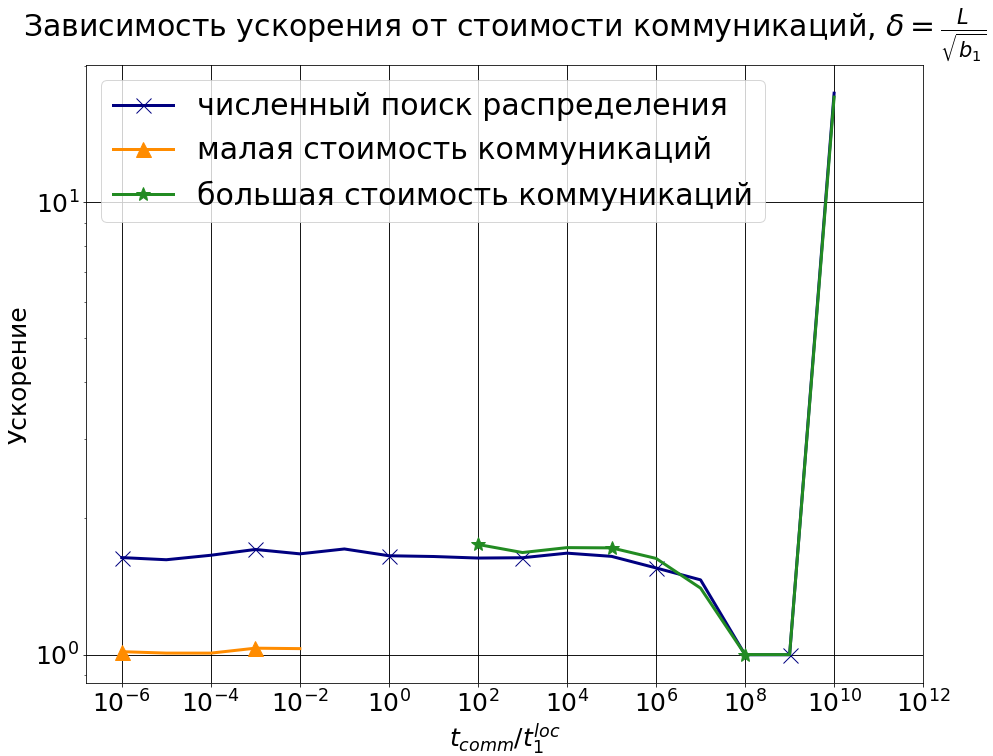
\includegraphics[scale = 0.24]{graph_rus11.png}}
    {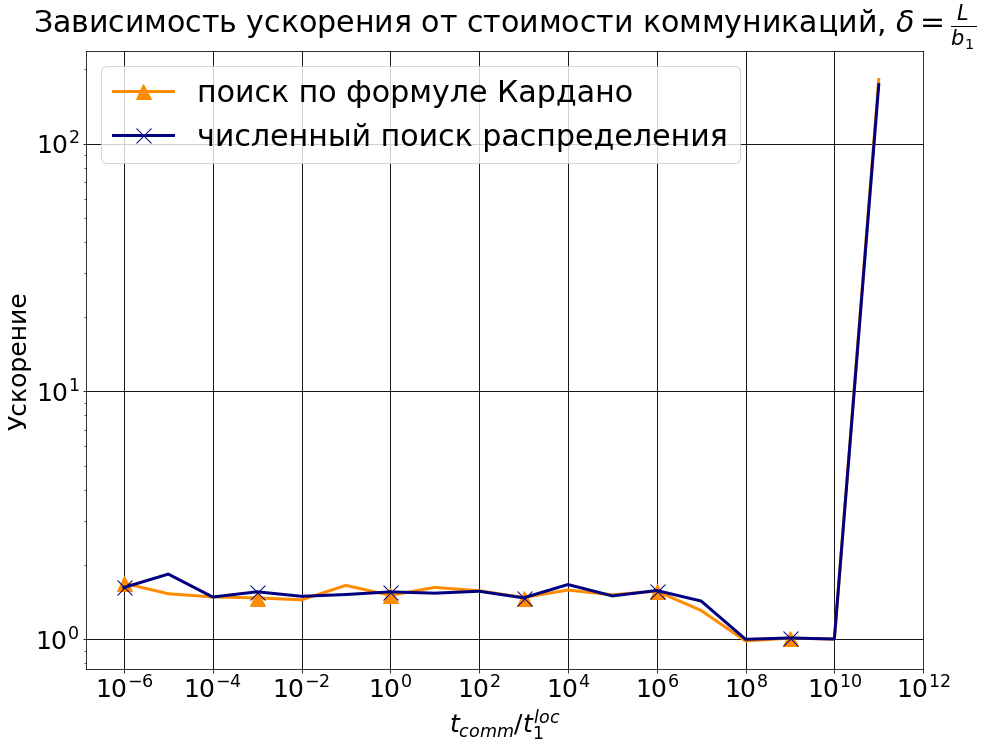
\includegraphics[scale = 0.24]{graph_rus12.png}}
    \caption{Эксперименты с распределением данных}
    \label{ris:image}
\end{figure}


%\begin{figure}[h]
%\center{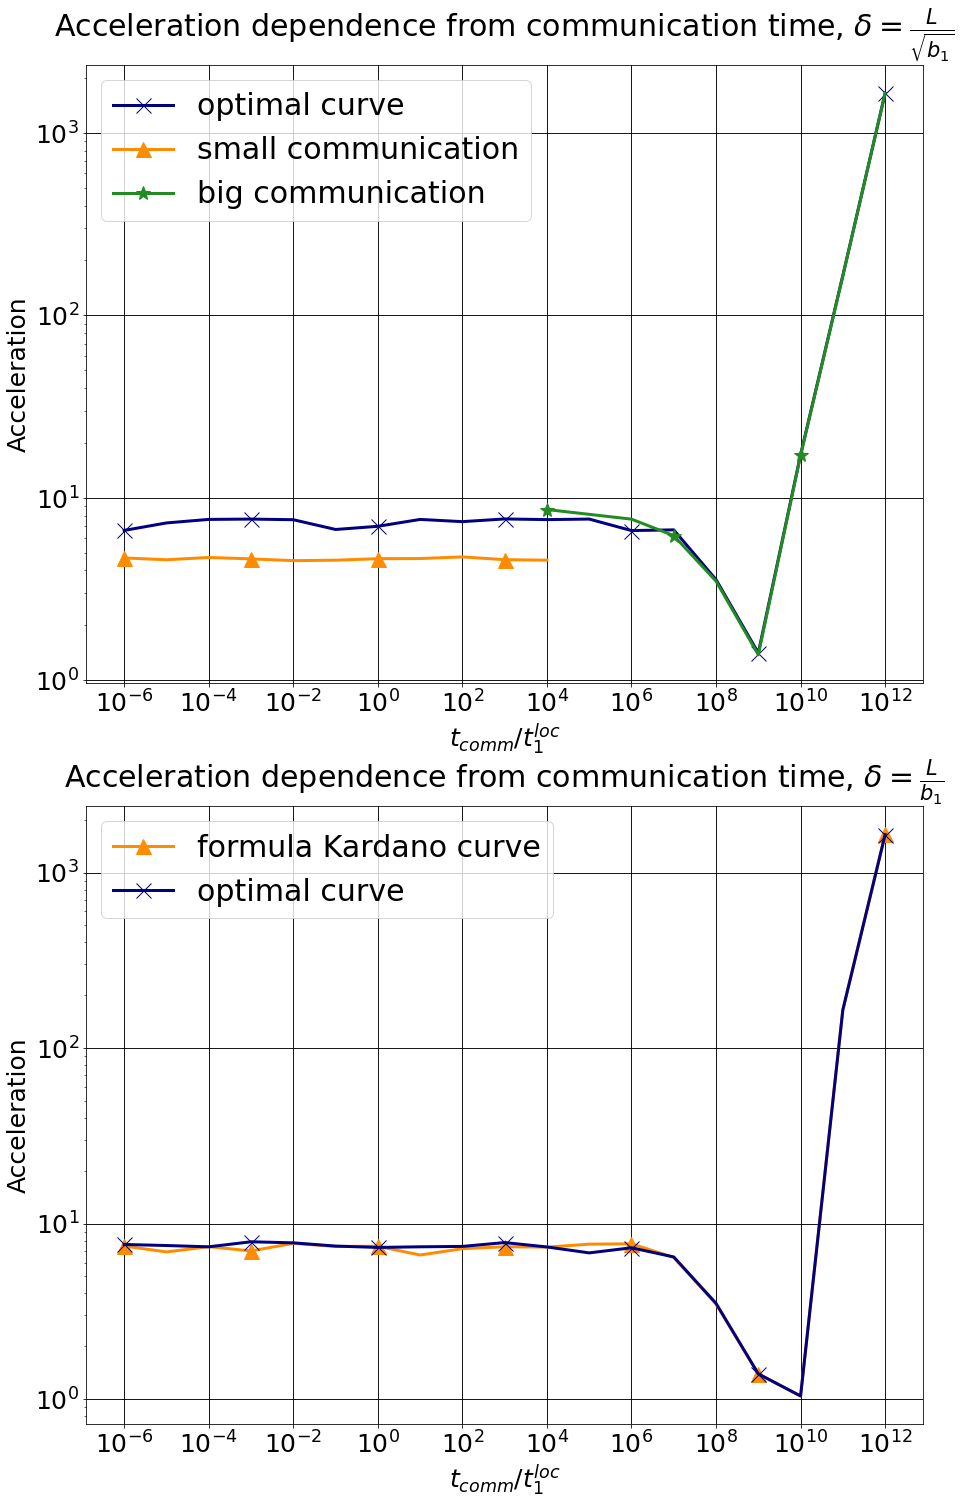
\includegraphics[width=0.8\linewidth]{final_graph.png}}
%\caption{Final results}
%\label{ris:image}
%\end{figure}

% \section*{5.2. Анализ}
% Проанализируем полученные графики. Формула для случая больших коммуникаций и формула Кардано практически совпали с поиском оптимального решения. Для случая малых коммуникаций результаты оказались хуже. Это объясняется тем, что формула была получена в грубом приближении. Но если учесть константы $\alpha, \beta$, то можно получить лучший результат, который приведен ниже.



% \begin{gather*}
%     F=\left(\max \left\{\tau_1^{loc} \cdot b_1 ;\left(N-b_1\right) \cdot\left(\sum_{i=2}^n \frac{1}{\tau_i^{loc}}\right)^{-1}\right\}+\tau_{comm}\right) \cdot \frac{\alpha}{\sqrt[4]{b_1}}+\tau_1^{loc} b_1 \cdot \beta \\
%     \text {Уже была проведена оценка того, что } b_1 \leq b_1^0 \Rightarrow F=\left(N-b_1\right)\cdot \left(\sum_{i=2}^n \frac{1}{\tau_i^{loc}}\right)^{-1} \cdot \frac{\alpha}{\sqrt[4]{b_1}}+\tau_1^{loc} b_1 \cdot \beta.
% \end{gather*}


% \begin{gather*}
%     F=N\left(\sum_{i=2}^n \frac{1}{\tau_i^{loc}}\right)^{-1} \alpha b^{-\frac{1}{4}}-\left(\sum_{i=2}^n \frac{1}{\tau_i^{loc}}\right)^{-1} \alpha b_1^{\frac{3}{4}}+\tau_1^{l o c} \beta b_1. \\
%     \text {Положим} \quad \alpha \sim 10^6, \beta \sim 10^9 \Rightarrow \\ 
%     F \cong 10^6 N \left(\sum_{i=2}^n \frac{1}{\tau_i^{loc}}\right)^{-1} \cdot b^{-\frac{1}{4}}-10^6 \left(\sum_{i=2}^n \frac{1}{\tau_i^{loc}}\right)^{-1} \cdot b_1^{\frac{3}{4}}+10^9 \tau_1^{loc} b_1, \\
%     \frac{1}{4} \cdot 10^6 N \left(\sum_{i=2}^n \frac{1}{\tau_i^{loc}}\right)^{-1} \cdot b_1^{-\frac{5}{4}} \ \leq 10^5 \tau_1^{loc} \Rightarrow b_1 \leq \frac{4 \cdot 10^3 \tau_1^{loc}}{N\left(\sum_{i=2}^n\left(\tau_i^{loc}\right)^{-1}\right)^{-1}}.
% \end{gather*}

\section*{5.2. Эксперименты с шумом}

Мы модифицировали моделирование алгоритма \ref{alg:1}, добавив шум в коммуникации и мощности устройств. Шум генерировался из равномерного распределения, и его величина составляла 10, 20, 30, 50 и 100 $\%$ соответственно от абсолютного значения времени коммуникаций и мощности устройств. В новой модели шума были проведены измерения времени выполнения задачи Гребневой регрессии (Ридж-регрессии) с полученным распределением данных и с равномерным распределением, получив ускорение, дающее правильное распределение данных. При этом проводились измерения математического ожидания затрат на коммуникации и мощности устройств, а впоследствии было  получено ускорение при этих ожидаемых значениях. Эксперименты проводились только в случае больших затрат на связь \hyperref[s:4.1]{4.1}. На рисунке \ref{ris:image2} приведен график отношения этих ускорений и доверительные интервалы.

\begin{figure}[!ht]
    \center{{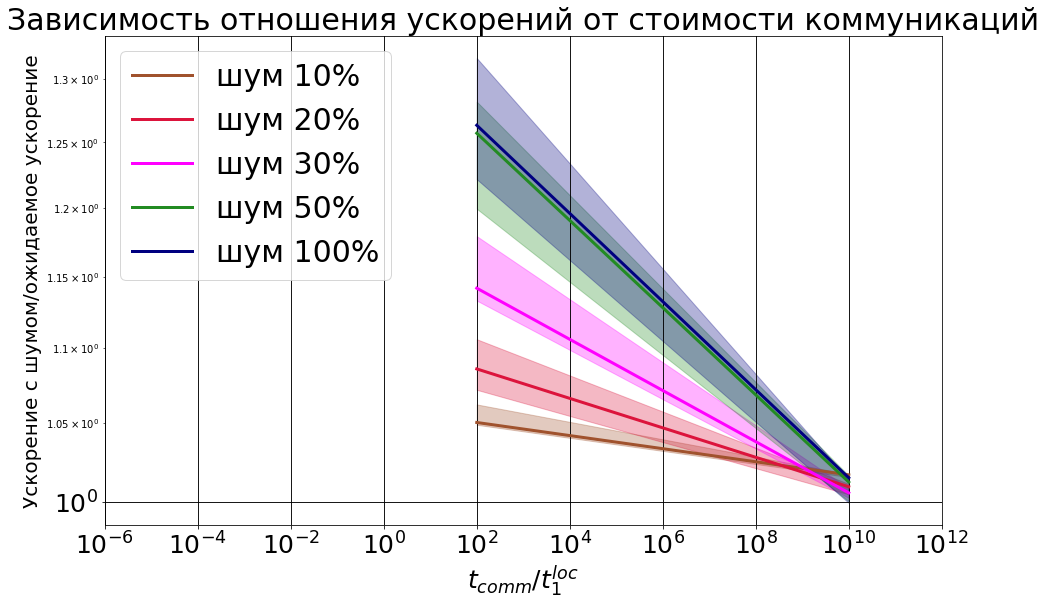
\includegraphics[scale = 0.35]{graph_noise_rus.png}}}
    \caption{Эксперименты с шумом в сети}
    \label{ris:image2}
\end{figure}

Проанализируем полученные результаты. Из графика видно, что все прямые попадают в доверительные интервалы, а значит для любого значения шума, приведенные в Секции \hyperref[s:4.1]{4.1} теоретические расчеты подтверждаются экспериментом. Также отметим, что вблизи значения $t_{comm}/t_1^{loc} = 10^{10}$ шум практически перестает влиять на результаты.

\section{Заключение}

В данной работе был представлен новый метод разбиения данных для задачи распределенной оптимизации. Новое решение основано на построении функции времени работы алгоритма \ref{alg:1} и нахождении ее минимума. Такой метод хорошо работает в сетях с различной стоимостью связи между сервером и локальными устройствами и различной мощностью устройств. Теоретические результаты были подтверждены экспериментально. Это показывает, что данный метод дает ускорение при решении такого рода задач. Кроме того, предполагая наличие шума в сетях, была найдена погрешность оптимального решения и проведены соответствующие эксперименты.

\section*{Источники Финансирования}
Исследования А. Безносикова были поддержаны Российским научным фондом (проект № 23-11-00229).

\printbibliography[heading=bibintoc,title={Источники}]


\end{document}